% Propósito: relacionar el recorrido longitudinal entre las ventanas y el
% helicotrema con la organización transversal de rampas, fluidos y membranas.
% Origen: descripción de la sección \ref{sec:u6-rampas-fluidos}. Esquema
% anatómico propio, simplificado y sin escala.
% Descripción accesible: el panel izquierdo muestra una cóclea desenrollada.
% La rampa vestibular parte de la ventana oval, se comunica con la rampa
% timpánica en el helicotrema y esta termina en la ventana redonda; la rampa
% media queda entre ambas. El panel derecho muestra un corte transversal con
% perilinfa arriba y abajo, endolinfa en la rampa media, membrana de Reissner,
% membrana basilar, membrana tectorial y órgano de Corti.
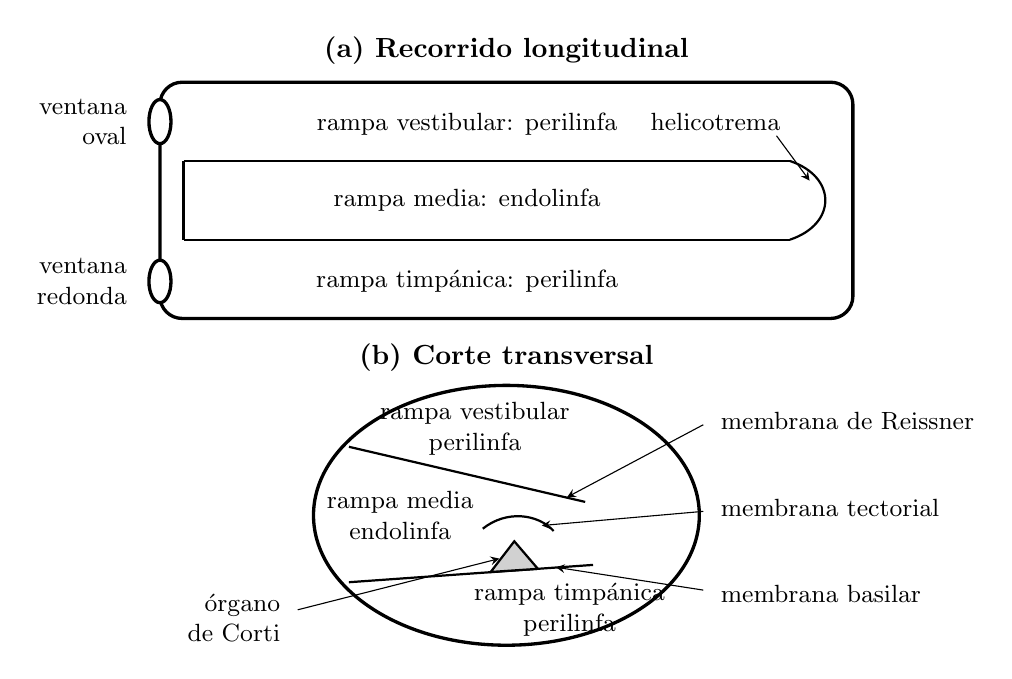
\begin{tikzpicture}[font=\small,>=stealth,x=1cm,y=1cm]
    % Panel longitudinal apilado: las tres rampas ocupan bandas separadas;
    % las ventanas se ubican en la base y el helicotrema en el extremo apical.
    \node[font=\bfseries] at (5.85,7.75) {(a) Recorrido longitudinal};
    \draw[very thick,rounded corners=8pt] (1.45,4.35) rectangle (10.25,7.35);
    \draw[thick] (1.75,6.35) -- (9.45,6.35);
    \draw[thick] (1.75,5.35) -- (9.45,5.35);
    \draw[thick] (9.45,6.35) .. controls (10.05,6.15) and (10.05,5.55) ..
        (9.45,5.35);
    \draw[thick] (1.75,6.35) -- (1.75,5.35);

    \node[align=center] at (5.35,6.82) {rampa vestibular: perilinfa};
    \node[align=center] at (5.35,5.85) {rampa media: endolinfa};
    \node[align=center] at (5.35,4.82) {rampa timpánica: perilinfa};

    \node[anchor=east] at (9.45,6.85) {helicotrema};
    \draw[->] (9.28,6.67) -- (9.70,6.10);

    \draw[very thick,fill=white] (1.45,6.85) ellipse (0.14 and 0.28);
    \draw[very thick,fill=white] (1.45,4.82) ellipse (0.14 and 0.27);
    \node[anchor=east,align=right] at (1.15,6.85) {ventana\\oval};
    \node[anchor=east,align=right] at (1.15,4.82) {ventana\\redonda};

    % Panel transversal apilado: las rampas se rotulan dentro del corte y las
    % llamadas de las membranas se ordenan en una columna exterior.
    \node[font=\bfseries] at (5.85,3.85) {(b) Corte transversal};
    \draw[very thick] (5.85,1.85) ellipse (2.45 and 1.65);
    \draw[thick] (3.85,2.72) -- (6.85,2.02);
    \draw[thick] (3.85,1.00) -- (6.95,1.22);

    \node[align=center] at (5.45,2.95)
        {rampa vestibular\\perilinfa};
    \node[align=center] at (4.50,1.85)
        {rampa media\\endolinfa};
    \node[align=center] at (6.65,0.65)
        {rampa timpánica\\perilinfa};

    \node[anchor=west,align=left] at (8.45,3.05)
        {membrana de Reissner};
    \draw[->] (8.35,3.00) -- (6.62,2.08);

    \draw[thick,fill=black!18] (5.65,1.13) -- (5.95,1.52)
        -- (6.25,1.17) -- cycle;
    \draw[thick] (5.55,1.68) .. controls (5.85,1.92) and (6.25,1.87) ..
        (6.45,1.65);

    \node[anchor=west,align=left] at (8.45,1.95)
        {membrana tectorial};
    \draw[->] (8.35,1.90) -- (6.30,1.72);

    \node[anchor=west,align=left] at (8.45,0.85)
        {membrana basilar};
    \draw[->] (8.35,0.90) -- (6.48,1.19);

    \node[anchor=east,align=right] at (3.10,0.55) {órgano\\de Corti};
    \draw[->] (3.20,0.65) -- (5.76,1.30);
\end{tikzpicture}
